
%%%%%%%%%%%%%%%%%%%%%%%%%%%%%%%%%%%%%%%%%%%%%%%%%%%%%%%%%%%%%%%%%%%%%%%%%%%%%%%
%%%
%%%                     SOLVE FOR THE VARIABLE(S)
%%%
%%%%%%%%%%%%%%%%%%%%%%%%%%%%%%%%%%%%%%%%%%%%%%%%%%%%%%%%%%%%%%%%%%%%%%%%%%%%%%%
\subsubsection*{Solve for The Variable}
\chead{Solve for the Variable}
\begin{tcolorbox}[title=Hint, colback=teal!10!white, colframe=teal!75!black]
Here are four approaches we used to solve these problems:
\begin{itemize}
\item  \textbf{Reduce to a single logarithm:} We used logarithm properties to simplify the equation to a single logarithm equal to a number. Then, we applied the definition property to solve for the variable.
\item  \textbf{Equate two logarithms:}We used logarithm properties to reduce the equation to two logarithms equal to each other. At that point, we set the arguments equal using the Equal Base Property and solved for the variable.\\

For both of the above methods, it's crucial to plug the result back into the original equation to verify that the equality holds. If it does, then the result is a valid solution; otherwise, it is not.
\item \textbf{Determine the domain first:} We first established the domain of the equation. Then, we used method one or two to solve for the variables and disregarded any solutions that fell outside the domain. This approach eliminates the need for back-substitution to verify the answers.
\item \textbf{Graphical method:} We graphed each side of the equation as separate functions (one for the left side and one for the right side). The intersection point(s) of these graphs represent the solutions. If no intersection points exist, then there are no solutions.\\

Problems 1-10 use the first two methods, and problems 11-17 use the third and fourth methods. 
\end{itemize}
\end{tcolorbox}



\newpage
\begin{enumerate}[resume]
\item  $2\log(8n+4)+6=10$
    {\color{blue}
    \begin{align*}
      2\log(8n+4)+6&=10\\
      2\log(8n+4)&=4\\
      \log(8n+4)&=2\\
      8n+4&=10^2\makebox[3cm]{\dotfill}\textit{Definition}\\
      8n&=96\\
      n&=12
    \end{align*}
Check the solution:
\begin{align*}
    2\log(8(12)+4)+6&\stackrel{?}{=}10\\
    2\log(100)+6&\stackrel{?}{=}10\\
    2\log(10^2)+6&\stackrel{?}{=}10\\
    2(2)+6&\stackrel{?}{=}10\makebox[3cm]{\dotfill}\textit{Inverse Rule}\\
    10&=10\, \checkmark
\end{align*}

\begin{tcolorbox}[title=Solution, colback=blue!10!white, colframe=blue!75!black]
$n=12$
\end{tcolorbox}
}

% ---------------------------------------------------------------------------------

\newpage
\item  $10-4\ln(9-8x)=6$
    {\color{blue}
    \begin{align*}
      10-4\ln(9-8x)&=6\\
      -4\ln(9-8x)&=-4\\
      \ln(9-8x)&=1\\
      9-8x&=e\makebox[3cm]{\dotfill}\textit{Definition or Identity Rule}\\
      x&=\dfrac{9-e}{8}
    \end{align*}
  Check the solution:
     \begin{align*}
      10-4\ln\left[9-8\left(\dfrac{9-e}{8}\right)\right]&\stackrel{?}{=}6\\
      10-4\ln\left(9-(9-e)\right)&\stackrel{?}{=}6\\
      10-4\ln\left(e\right)&\stackrel{?}{=}6\\
      10-4(1)&\stackrel{?}{=}6\makebox[3cm]{\dotfill}\textit{Identity Rule}\\
     10-4&\stackrel{?}{=}6\, \checkmark
    \end{align*}
    
\begin{tcolorbox}[title=Solution, colback=blue!10!white, colframe=blue!75!black]
$x=\dfrac{9-e}{8}$
\end{tcolorbox}
}
% ---------------------------------------------------------------------------------

\newpage
\item  $4+\log2(9k)=2$
    {\color{blue}
    \begin{align*}
        4+\log_2(9k)&=2\\
        \log_2(9k)&=-2\\
        9k&=2^{-2}\makebox[3cm]{\dotfill}\textit{Definition}\\
        9k&=\dfrac{1}{4}\\
        k&=\dfrac{1}{9\times 4}\\
        k&=\dfrac{1}{36}
    \end{align*}
Check the solution:
\begin{align*}
        4+\log2(9k)&\stackrel{?}{=}2\\
        4+\log2\left[9\left(\dfrac{1}{36}\right)\right]&\stackrel{?}{=}2\\
        4+\log2\left(\dfrac{1}{4}\right)&\stackrel{?}{=}2\\
        4+\log2\left(\dfrac{1}{2^2}\right)&\stackrel{?}{=}2\\
        4+\log2\left(2^{-2}\right)&\stackrel{?}{=}2\\
        4-2&\stackrel{?}{=}2\makebox[3cm]{\dotfill}\textit{Identity Rule}\\
        2&\stackrel{?}{=}2\,\checkmark
    \end{align*}
    
\begin{tcolorbox}[title=Solution, colback=blue!10!white, colframe=blue!75!black]
$k=\dfrac{1}{36}$
\end{tcolorbox}
}

% ---------------------------------------------------------------------------------

\newpage
\item  $\ln(-3x)=\ln(x^2-6x)$
    {\color{blue}
    \begin{align*}
       \ln(-3x)&=\ln(x^2-6x)\makebox[3cm]{\dotfill}\textit{Equality Base Rule}\\
       -3x&=x^2-6x\\
       x^2-3x&=0\\
       x(x-3)&=0\\
       x=0,&\quad x=3
    \end{align*}
    
Check the two values for $x$:   
 
   Check  $x=0$:
    \begin{align*}
       \ln(-3(0))&\stackrel{?}{=}\ln((0)^2-6(0))\\
       \ln(0)&\stackrel{?}{=}\ln(0)
    \end{align*}
    $\ln(0)$ is undefined. $x=0$ is not a solution

   Check  $x=3$:
    \begin{align*}
       \ln(-3(3))&\stackrel{?}{=}\ln((3)^2-6(3))\\
       \ln(-9))&\stackrel{?}{=}\ln(9-18)\\
       \ln(-9))&\stackrel{?}{=}\ln(-9)
    \end{align*}
        $\ln(-9)$ is undefined. $x=3$ is not a solution



\begin{tcolorbox}[title=Solution, colback=blue!10!white, colframe=blue!75!black]
No solutions
\end{tcolorbox}
}

% ---------------------------------------------------------------------------------

\newpage
\item  $\log_9(2n^2-14n)=\log_9(-45+n^2)$
    {\color{blue}
    \begin{align*}
        \log_9(2n^2-14n)&=\log_9(-45+n^2)\\
        2n^2-14n&=-45+n^2\\
        n^2-14n+45&=0\\
        (n-9)(n-5)&=0\\
        n-9=0,&\quad n-5=0\\
        n=9&\quad n=5
    \end{align*}

Check the two values for $x$:   

 Check $n=9$:
    \begin{align*}
        \log_9(2(9)^2-14(9))&\stackrel{?}{=}\log_9(-45+(9)^2)\\
        \log_9(2\times 81-126)&\stackrel{?}{=}\log_9(-45+81)\\
        \log_9(162-131)&\stackrel{?}{=}\log_9(-45+81)\\
        \log_9(36)&\stackrel{?}{=}\log_9(36)\,\checkmark
    \end{align*}
$x=9$ is a solution.

 Check $n=5$:
    \begin{align*}
        \log_9(2(5)^2-14(5))&\stackrel{?}{=}\log_9(-45+(5)^2)\\
        \log_9(2\times 25-70)&\stackrel{?}{=}\log_9(-45+25)\\
        \log_9(50-70)&\stackrel{?}{=}\log_9(-20)\\
        \log_9(-20)&\stackrel{?}{=}\log_9(-20)\,\times
    \end{align*}
    $x=5$ is not a solution since $\log_9(-20)$ is not defined. 

\vspace{0.5in}    
 \begin{tcolorbox}[title=Solution, colback=blue!10!white, colframe=blue!75!black]
$x=9$
\end{tcolorbox}   
    }

% ---------------------------------------------------------------------------------

\newpage
\item  $\log(x+12)=\log(x)+\log(12)$
    {\color{blue}
    \begin{align*}
        \log(x+12)&=\log(x)+\log(12)\\
        \log(x+12)&=\log\left(12\cdot x\right)\\
        x+12&=12x\\
        11x&=12\\
        x&=\frac{12}{11}
    \end{align*}

Check answer:

    \begin{align*}
        \log\left(\frac{12}{11}+12\right)&\stackrel{?}{=}\log\left(\frac{12}{11}\right)+\log(12)\\
        \log\left(\frac{12+11\times 12}{11}+12\right)&\stackrel{?}{=}\log\left(\frac{12}{11}\times 12\right)\\
        \log\left(\frac{12+11\times 12}{11}\right)&\stackrel{?}{=}\log\left(\frac{144}{11}\right)\\
        \log\left(\frac{144}{11}\right)&\stackrel{?}{=}\log\left(\frac{144}{11}\right)\,\checkmark\\
    \end{align*}
    

\begin{tcolorbox}[title=Solution, colback=blue!10!white, colframe=blue!75!black]
$x=\dfrac{12}{11}$
\end{tcolorbox}
}
    
% ---------------------------------------------------------------------------------

\newpage
\item  $\ln(x)+\ln(x-3)=\ln(7x)$
    {\color{blue}
    \begin{align*}
        \ln(x)+\ln(x-3)&=\ln(7x)\\
        \ln\left(x\cdot(x-3)\right)&=\ln(7x)\\
        x(x-3)&=7x\\
        x^2-3x-7x&=0\\
        x(x-10)&=0\\
        x=0&\quad x-10=0\\
        x=0&\quad x=10
    \end{align*}
    
Check the two values for $x$:   

check $x=0$:
    \begin{align*}
        \ln(0)+\ln(0-3)&\stackrel{?}{=}\ln(7\times 0)\\
        \ln(0)+\ln(-3)&\stackrel{?}{=}\ln(0)\\
    \end{align*}
$\ln(0)$ and $\ln(-3)$ are undefined so $x=0$ is not a solution.


check $x=10$:
    \begin{align*}
        \ln(10)+\ln(10-3)&\stackrel{?}{=}\ln(7\times 10)\\
        \ln(10)+\ln(7)&\stackrel{?}{=}\ln(70)\\
        \ln(10\times 7)&\stackrel{?}{=}\ln(70)\\
        \ln(70)&\stackrel{?}{=}\ln(70)\,\checkmark
    \end{align*}



\begin{tcolorbox}[title=Solution, colback=blue!10!white, colframe=blue!75!black]
$x=10$
\end{tcolorbox}
}

% ---------------------------------------------------------------------------------

\newpage
\item  $\ln(7)+\ln(2-4x^2)=\ln(14)$

    {\color{blue}
    \begin{align*}
        \ln(7)+\ln(2-4x^2)&=\ln(14)\\
        \ln\left(7\cdot (2-4x^2)\right)&=\ln(14)\\
        7(2-4x^2)&=14\\
        2-4x^2&=2\\
        -4x^2&=0\\
        x&=0
    \end{align*}

Check answer:


    \begin{align*}
        \ln(7)+\ln(2-4(0)^2)&\stackrel{?}{=}\ln(14)\\
        \ln(7)+\ln(2)&\stackrel{?}{=}\ln(14)\\
        \ln(7\times 2)&\stackrel{?}{=}\ln(14)\\
        \ln(14)&\stackrel{?}{=}\ln(14)\,\checkmark
    \end{align*}

\begin{tcolorbox}[title=Solution, colback=blue!10!white, colframe=blue!75!black]
$x=0$
\end{tcolorbox}
}
    
% ---------------------------------------------------------------------------------

\newpage
\item  $\log_8(x+6)-\log_8(x)=\log_8(58)$
    {\color{blue}
    \begin{align*}
        \log_8(x+6)-\log_8(x)&=\log_8(58)\\
        \log_8\left(\dfrac{x+6}{x}\right)&=\log_8(58)\\
        \dfrac{x+6}{x}&=58\\
        x+6&=58x\\
        57x&=6\\
        x&=\frac{6}{57}
    \end{align*}


Check answer:

    \begin{align*}
        \log_8\left(\dfrac{6}{57}+6\right)-\log_8\left(\dfrac{6}{57}\right)&\stackrel{?}{=}\log_8(58)\\
        \log_8\left(\dfrac{6+57\times 6}{57}\right)-\log_8\left(\dfrac{6}{57}\right)&\stackrel{?}{=}\log_8(58)\\
        \log_8\left(\dfrac{58\times 6}{57}\right)-\log_8\left(\dfrac{6}{57}\right)&\stackrel{?}{=}\log_8(58)\\
         \log_8\left(\dfrac{\dfrac{58\times 6}{57}}{\dfrac{6}{57}}\right)
         &\stackrel{?}{=}\log_8(58)\\     
        \log_8(58)&\stackrel{?}{=}\log_8(58)\,\checkmark
    \end{align*}

\begin{tcolorbox}[title=Solution, colback=blue!10!white, colframe=blue!75!black]
$x=\frac{6}{57}$
\end{tcolorbox}

    }
    
% ---------------------------------------------------------------------------------

\newpage
\item  $\ln(3)-\ln(3-3x)=\ln(4)$
    {\color{blue}
    \begin{align*}
        \ln(3)-\ln(3-3x)&=\ln(4)\\
        \ln\left(\dfrac{3}{3-3x}\right)&=\ln(4)\\
        \ln\left(\dfrac{1}{1-x}\right)&=\ln(4)\\  
        \dfrac{1}{1-x}&=4\\
        1-x&=\frac{1}{4}\\
        x&=1-\frac{1}{4}\\
        x&=\frac{3}{4}
    \end{align*}

Check answer:   
 
    \begin{align*}
        \ln(3)-\ln\left(3-3\left(\dfrac{3}{4}\right)\right)&\stackrel{?}{=}\ln(4)\\
        \ln(3)-\ln\left(3-\dfrac{9}{4}\right)&\stackrel{?}{=}\ln(4)\\
        \ln(3)-\ln\left(\dfrac{4\times 3-9}{4}\right)&\stackrel{?}{=}\ln(4)\\
        \ln(3)-\ln\left(\dfrac{12-9}{4}\right)&\stackrel{?}{=}\ln(4)\\
        \ln(3)-\ln\left(\dfrac{3}{4}\right)&\stackrel{?}{=}\ln(4)\\
        \ln(3)-\left[\ln(3)-\ln(4)\right]&\stackrel{?}{=}\ln(4)\\
        \ln(3)-\ln(3)+\ln(4)&\stackrel{?}{=}\ln(4)\\
        \ln(4)&\stackrel{?}{=}\ln(4)\,\checkmark
    \end{align*}


\begin{tcolorbox}[title=Solution, colback=blue!10!white, colframe=blue!75!black]
$x=\dfrac{3}{4}$
\end{tcolorbox}
}
    
  
% ---------------------------------------------------------------------------------

\newpage
\item  $2\log_4(x) = \log_4(9)$
{\color{blue}
    
    Let's look at the domain first: \\
    $\log_4(x): x > 0$\\

    The domain is $x>0$ as shown in the figure below: 
    
    \begin{figure}[!h]
    \centering
    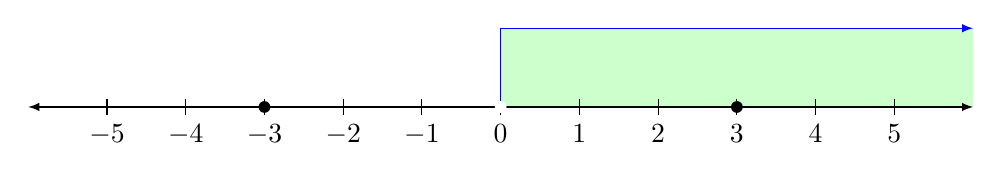
\begin{tikzpicture}
        \fill[green!20](6,0)rectangle(0,1);
        \draw[latex-latex] (-6,0) -- (6,0) ;
        \foreach \x in {-5,-4,-3,-2,-1,0,1,2,3,4,5} \draw[shift={(\x,0)},color=black] (0pt,3pt) -- (0pt,-3pt) node[below] {$\x$};
        \node[circle,fill=white,inner sep=1.5pt](a)at(0,0){};
        \node[circle,fill=black,inner sep=1.5pt](b)at(3,0){};
        \node[circle,fill=black,inner sep=1.5pt](c)at(-3,0){};
        \draw[-latex,blue](a)--++(0,1)--++(6,0);
    \end{tikzpicture}
    \caption{The domain is the green shaded area}
    \end{figure}
    Solve for $x$
    \begin{align*}
        2\log_4(x) &= \log_4(9)\\
        \log_4(x^2) &= \log_4(9))\\
        x^2&=9\\
        x&=\pm\sqrt{9}=\pm 3\\
    \end{align*}
    
    Ignore $x=-3$ since it's not in the domain of the problem. The only solution is $x=3$ and is verified graphically below.
    }
    \begin{figure}[htbp]
        \centering
        \includegraphics[width=0.6\textwidth]{log1_1}
        \caption{The solution to the problem is the intersection between $2\log_4(x) = \log_4(9)$}
        %\label{fig:myimage}
    \end{figure}


\begin{tcolorbox}[title=Solution, colback=blue!10!white, colframe=blue!75!black]
$x=3 $
\end{tcolorbox}

%     \begin{tcolorbox}[ams align*, colback=orange!60, colframe=blue]
% \text{The solution to the above equation is x=3 }
% \end{tcolorbox}

\newpage


    \item   $\log_2(x-1) - \log_2(x+1) = \log_2(3)$
    {\color{blue}
    \begin{align*}
       \log_2(x-1) - \log_2(x+1) &= \log_2(3) \\
       \log_2\left(\dfrac{x-1}{x+1}\right)&=\log_2(3)\\
       \dfrac{x-1}{x+1}&=3\\
       x-1&=3(x+1)\\
       x-1&=3x+3\\
       -4&=2x\\
       x&=-2
    \end{align*}
    }

    \begin{figure}[!h]
    \centering
    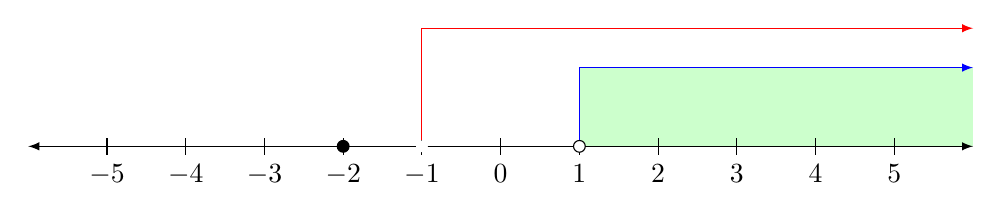
\begin{tikzpicture}
        \fill[green!20](6,0)rectangle(1,1);
        \draw[latex-latex] (-6,0) -- (6,0) ;
        \foreach \x in {-5,-4,-3,-2,-1,0,1,2,3,4,5} \draw[shift={(\x,0)},color=black] (0pt,3pt) -- (0pt,-3pt) node[below] {$\x$};
        \node[circle,fill=white,inner sep=1.5pt](a)at(-1,0){};
        \node[circle,draw,fill=white,inner sep=1.5pt](b)at(1,0){};
        \node[circle,draw,fill=black,inner sep=1.5pt](c)at(-2,0){};
        \draw[-latex,red](a)--++(0,1.5)--++(7,0);
        \draw[-latex,blue](b)--++(0,1)--++(5,0);
    \end{tikzpicture}
    \caption{The domain is the green shaded area}
    \end{figure}

    $x=-2$ is obviously not in the domain, so this problem does not any real solutions. 

\begin{tcolorbox}[title=Solution, colback=blue!10!white, colframe=blue!75!black]
No real solutions. 
\end{tcolorbox}


% \begin{tcolorbox}[ams align*, colback=orange!60, colframe=blue]
% \text{There are no real solutions to this problem.}
% \end{tcolorbox}

        
% \begin{tikzpicture}

% % Draw the number line with arrows
% \draw[<->, >=stealth] (-4,0) -- (4,0) node[below] {$x$};

% % Add tick marks and labels
% \foreach \x in {-3, -2, -1, 0, 1, 2, 3} {
%   \draw[shift={(\x,0)}, color=black] (0pt,3pt) -- (0pt,-3pt) node[below] {$\x$};
% }

% % Draw the domain for a specific example, e.g., [1, 3)
% % Replace with your specific domain and endpoints
% \draw[line width=2pt, blue] (1,0) node[circle, fill=blue, inner sep=1pt] {} -- (3,0) node[circle, fill=white, draw=blue, inner sep=1pt] {};

% \end{tikzpicture}

\newpage
    \item   $\log_3(x) + \log_3(x+2) = \log_3(15)$:\\
    {\color{blue}
    
    Let's look at the domain first: \\
    $\log_3(x): x > 0$\\
    $\log_3(x+2): x > -2$

    The overall domain is $x>0$ as shown in the figure below: 
    
    \begin{figure}[!h]
    \centering
    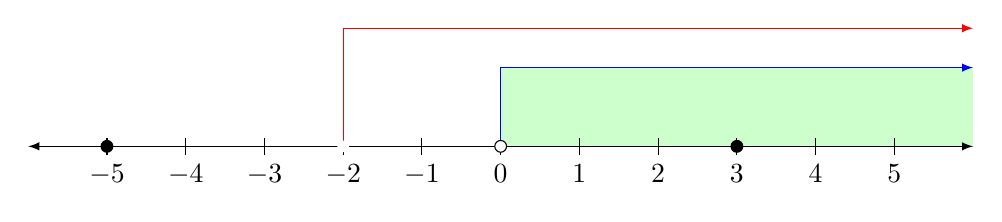
\begin{tikzpicture}
        \fill[green!20](6,0)rectangle(0,1);
        \draw[latex-latex] (-6,0) -- (6,0) ;
        \foreach \x in {-5,-4,-3,-2,-1,0,1,2,3,4,5} \draw[shift={(\x,0)},color=black] (0pt,3pt) -- (0pt,-3pt) node[below] {$\x$};
        \node[circle,fill=white,inner sep=1.5pt](a)at(-2,0){};
        \node[circle,draw,fill=white,inner sep=1.5pt](b)at(0,0){};
        \node[circle,draw,fill=black,inner sep=1.5pt](c)at(3,0){};
        \node[circle,draw,fill=black,inner sep=1.5pt](d)at(-5,0){};

        \draw[-latex,red](a)--++(0,1.5)--++(8,0);
        \draw[-latex,blue](b)--++(0,1)--++(6,0);
    \end{tikzpicture}
    \caption{The domain is the green shaded area}
    \end{figure}

    \begin{align*}
        \log_3(x) + \log_3(x+2) &= \log_3(15)\\
        \log_3(x(x+2))&=\log_3(15)\\
        x(x+2)&=15\\
        x^2+2x-15&=0\\
        (x+5)(x-3)&=0\\
        x&=-5;x=3
    \end{align*}
    
    Ignore $x=-5$ since it's not in the domain of the problem
    }
    \begin{figure}[htbp]
        \centering
        \includegraphics[width=0.6\textwidth]{log1_1}
        \caption{The solution to the problem is the intersection between $\log_3(x)+\log_3(x+2)$ and $\log_3(15)$}
        %\label{fig:myimage}
    \end{figure}

\begin{tcolorbox}[title=Solution, colback=blue!10!white, colframe=blue!75!black]
$x=3 $
\end{tcolorbox}

%     \begin{tcolorbox}[ams align*, colback=orange!60, colframe=blue]
% \text{The solution to the above equation is x=3 }
% \end{tcolorbox}

\newpage

    \item   $\log_5(x+3) + \log_5(x-3) = \log_5(16)$:
    {\color{blue}
  
    Let's look at the domain first: \\
    $\log_3(x+3): x > -3$\\
    $\log_3(x-3): x > 3$

    The overall domain is $x>3$ as shown in the figure below: 
    
    \begin{figure}[!h]
    \centering
    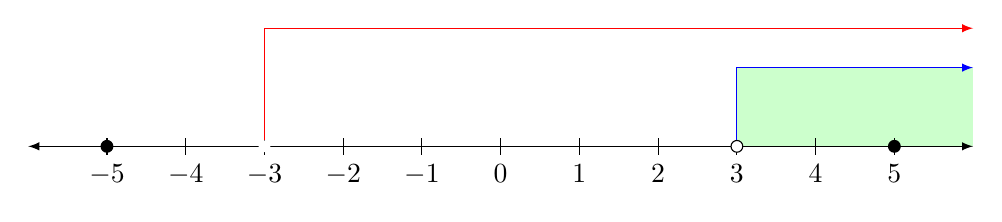
\begin{tikzpicture}
        \fill[green!20](6,0)rectangle(3,1);
        \draw[latex-latex] (-6,0) -- (6,0) ;
        \foreach \x in {-5,-4,-3,-2,-1,0,1,2,3,4,5} \draw[shift={(\x,0)},color=black] (0pt,3pt) -- (0pt,-3pt) node[below] {$\x$};
        \node[circle,fill=white,inner sep=1.5pt](a)at(-3,0){};
        \node[circle,draw,fill=white,inner sep=1.5pt](b)at(3,0){};
        \node[circle,draw,fill=black,inner sep=1.5pt](c)at(5,0){};
        \node[circle,draw,fill=black,inner sep=1.5pt](d)at(-5,0){};
        \draw[-latex,red](a)--++(0,1.5)--++(9,0);
        \draw[-latex,blue](b)--++(0,1)--++(3,0);
    \end{tikzpicture}
    \caption{The domain is the green shaded area}
    \end{figure}

    \begin{align*}
        \log_5(x) + \log_5(x+2) &= \log_5(16)\\
        \log_5((x+3)(x-3))&=\log_5(16)\\
        (x+3)(x-3)&=16\\
        x^2-9&=16\\
        x^2&=25\\
        x&=\pm\sqrt{25}=\pm 5
    \end{align*}
    
    Ignore $x=-5$ since it's not in the domain of the problem
    }
    \begin{figure}[htbp]
        \centering
        \includegraphics[width=0.6\textwidth]{log1_2}
        \caption{The solution to the problem is the intersection between $\log_5(x+3) + \log_5(x-3)$ and $\log_5(16)$}
        %\label{fig:myimage}
    \end{figure}


\begin{tcolorbox}[title=Solution, colback=blue!10!white, colframe=blue!75!black]
$x=5 $
\end{tcolorbox}

%     \begin{tcolorbox}[ams align*, colback=orange!60, colframe=blue]
% \text{The solution to the above equation is x=5 }
% \end{tcolorbox}

\newpage
    \item  $\log_{x-1}(x+1) + \log_{x+1}(x-1) = \frac{5}{2}$
    
    {\color{blue}
    Let's look at the domain first. The base of the log and the argument must both be positive: \\
    $x+1>0\Rightarrow   x > -1$\\
    $x-1>0\Rightarrow  x>-1$

    The overall domain is $x>1$ as shown in the figure below: 
    
    \begin{figure}[!h]
    \centering
    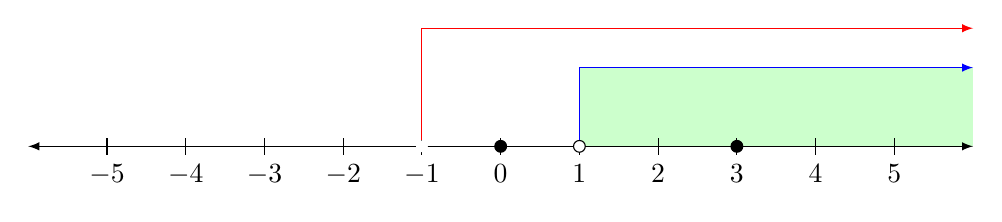
\begin{tikzpicture}
        \fill[green!20](6,0)rectangle(1,1);
        \draw[latex-latex] (-6,0) -- (6,0) ;
        \foreach \x in {-5,-4,-3,-2,-1,0,1,2,3,4,5} \draw[shift={(\x,0)},color=black] (0pt,3pt) -- (0pt,-3pt) node[below] {$\x$};
        \node[circle,fill=white,inner sep=1.5pt](a)at(-1,0){};
        \node[circle,draw,fill=white,inner sep=1.5pt](b)at(1,0){};
        \node[circle,draw,fill=black,inner sep=1.5pt](c)at(0,0){};
        \node[circle,draw,fill=black,inner sep=1.5pt](d)at(3,0){};
        \draw[-latex,red](a)--++(0,1.5)--++(7,0);
        \draw[-latex,blue](b)--++(0,1)--++(5,0);
    \end{tikzpicture}
    \caption{The domain is the green shaded area}
    \end{figure}

    Now let's solve the problem analytically and verify the solutions algebraically and graphically
    \begin{align*}
        \log_{x-1}(x+1) + \log_{x+1}(x-1) &= \frac{5}{2}\\
        \dfrac{\log_{x+1}(x+1)}{\log_{x+1}(x-1)}+\log_{x+1}(x-1)&=\frac{5}{2}\makebox[3cm]{\dotfill}\textit{Change of base}\\
        \dfrac{1}{\log_{x+1}(x-1)}+\log_{x+1}(x-1)&=\frac{5}{2}\makebox[3cm]{\dotfill}\textit{Identity Rule}\\
        1+\left(\log_{x+1}(x-1)\right)^2=\frac{5}{2}\log_{x+1}(x-1)\\
        \left(\log_{x+1}(x-1)\right)^2-\frac{5}{2}\log_{x+1}(x-1)+1=0\\
    \end{align*}
    We have a quadratic form. One way to solve it analytically is by doing a variable substitution. 
Let $u=\log_{x+1}(x-1)$
    \begin{align*}
        \left(\log_{x+1}(x-1)\right)^2-\frac{5}{2}\log_{x+1}(x-1)+1&=0\\
        u^2-\frac{5}{2}u+1&=0\\
        2u^2-5u+2&=0\\
        (2u-1)(u-2)&=0\\
        2u-1=0 ;&\quad u-2=0\\
        u=\frac{1}{2};&\quad u=2
    \end{align*}
We have two real solutions to the above quadratic formula:  $u=u_1=2$ or $u=u_2=\frac{1}{2}$. Now solve for $x$ for each value of $u$:
    \begin{align*}
        \log_{x+1}(x-1)&=u_1\\
        \log_{x+1}(x-1)&=2\\
        x-1&=(x+1)^2\\
        x-1&=x^2+2x+1\\
        x^2+x+2&=0
    \end{align*}

    The discriminant of the above quadratic equation is negative: 
    \[
        D=b^2-4ac=1^2-4(1)(1)=-3<0
    \]
    This means that $\log_{x+1}(x-1)=2$ has no real solutions. 
    
    Let's look at the other value of $u$:
    \begin{align*}
        \log_{x+1}(x-1)&=u_2\\
        \log_{x+1}(x-1)&=\frac{1}{2}\\
        x-1&=(x+1)^{1/2}\\
        x^2-2x+1&=x+1\\
        x^2-3x&=0\\
        x(x-3)&=0
    \end{align*}
We ignore $x=0$ since it's not in the domain. $x=3$ seems to be the only solution. Verify it algebraically:
    \begin{align*}
        \log_{x-1}(x+1) + \log_{x+1}(x-1) &= \frac{5}{2}\\
        \log_{3-1}(3+1) + \log_{3+1}(3-1)&\stackrel{?}{=}\frac{5}{2}\\
        \log_2(4)+\log_4(2)&\stackrel{?}{=}\frac{5}{2}\\
        \log_2(2^2)+\frac{1}{\log_2(4)}&\stackrel{?}{=}\frac{5}{2}\\
        \log_2(2^2)+\frac{1}{\log_2(2^2)}&\stackrel{?}{=}\frac{5}{2}\\
        2+\frac{1}{2} &\stackrel{?}{=}\frac{5}{2}\makebox[3cm]{\dotfill}\textit{TRUE}\\
    \end{align*}


        \begin{figure}[htbp]
        \centering
        \includegraphics[width=0.9\textwidth]{log1_3}
        \caption{Graphical solution to the equation $\log_{x-1}(x+1) + \log_{x+1}(x-1) = \frac{5}{2}$, which is the zero of the function.}
        %\label{fig:myimage}
    \end{figure}


\begin{tcolorbox}[title=Solution, colback=blue!10!white, colframe=blue!75!black]
$x=3 $
\end{tcolorbox}

%     \begin{tcolorbox}[ams align*, colback=orange!60, colframe=blue]
% \text{The solution to }\log_{x-1}(x+1) + \log_{x+1}(x-1) = \frac{5}{2} \text{ is } x=3 
% \end{tcolorbox}
}

\newpage
\item  $(\log_2(x))^2 - 5\log_2(x) + 6 = 0$:
      {\color{blue}
    
    Let's look at the domain first: \\
    $\log_2(x): x > 0$\\

    The domain is $x>0$ as shown in the figure below: 
    
    \begin{figure}[!h]
    \centering
    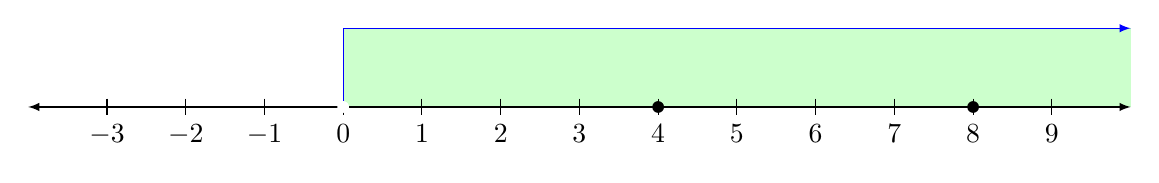
\begin{tikzpicture}
        \fill[green!20](10,0)rectangle(0,1);
        \draw[latex-latex] (-4,0) -- (10,0) ;
        \foreach \x in {-3,-2,-1,0,1,2,3,4,5,6,7,8,9} \draw[shift={(\x,0)},color=black] (0pt,3pt) -- (0pt,-3pt) node[below] {$\x$};
        \node[circle,fill=white,inner sep=1.5pt](a)at(0,0){};
        \node[circle,fill=black,inner sep=1.5pt](b)at(4,0){};
        \node[circle,fill=black,inner sep=1.5pt](c)at(8,0){};
        \draw[-latex,blue](a)--++(0,1)--++(10,0);
    \end{tikzpicture}
    \caption{The domain is the green shaded area}
    \end{figure}
 We have a quadratic form. One way to solve it analytically is by doing a variable substitution.     
 Let $u=\log_2(x)$
 \begin{align*}
        (\log_2(x))^2 - 5\log_2(x) + 6 &= 0
        u^2 - 5u + 6 = 0\\
        (u-3)(u-2)&=0\\
        u-3=0;&\quad u-2=0\\
        u=3&\quad u=32
    \end{align*}

   We have two real solutions to the above quadratic formula:  $u=u_1=3$ or $u=u_2=2$. Now solve for $x$ for each value of $u$:
    \begin{align*}
        \log_2(x)&=u_1\\
        \log_2(x)&=3\\
        x&=2^3\\
        x&=8
    \end{align*}
    \begin{align*}
        \log_2(x)&=u_2\\
        \log_2(x)&=4\\
        x&=2^2\\
        x&=4
    \end{align*}
    Both values of $x$ are acceptable since they are in the domain the function (they both lay in the gree region in the graph above).This is also verified graphically below:
    \newpage
    }
    \begin{figure}[htbp]
        \centering
        \includegraphics[width=0.8\textwidth]{log1_5}
        \caption{The solutions to the problem are the zeros of the function  $f(x)=(\log_2(x))^2 - 5\log_2(x) + 6 $}
        %\label{fig:myimage}
    \end{figure}

\begin{tcolorbox}[title=Solution, colback=blue!10!white, colframe=blue!75!black]
$x=4$ and $x=8$
\end{tcolorbox}

%     \begin{tcolorbox}[ams align*, colback=orange!60, colframe=blue]
% \text{The solutions to the above function are x=4 and x=8 }
% \end{tcolorbox}
    
\newpage
    \item  $\log_x(x+6) = \log_{x+6}(x) + \frac{1}{2}$
    {\color{blue}
    
    Let's look at the domain first: \\
    $ x > 0$\\
    $x+6>0\Rightarrow  x > -6$\\


    The domain is $x>0$ as shown in the figure below: 
    
    \begin{figure}[!h]
    \centering
    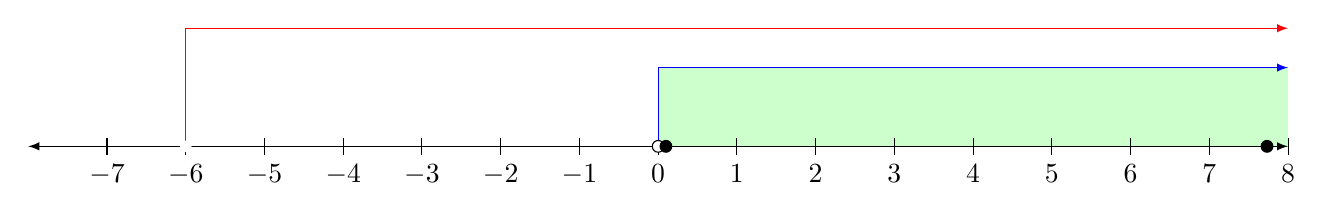
\begin{tikzpicture}
        \fill[green!20](8,0)rectangle(0,1);
        \draw[latex-latex] (-8,0) -- (8,0) ;
        \foreach \x in {-7,-6,-5,-4,-3,-2,-1,0,1,2,3,4,5,6,7,8} \draw[shift={(\x,0)},color=black] (0pt,3pt) -- (0pt,-3pt) node[below] {$\x$};
        \node[circle,fill=white,inner sep=1.5pt](a)at(-6,0){};
        \node[circle,draw,fill=white,inner sep=1.5pt](b)at(0,0){};
        \node[circle,draw,fill=black,inner sep=1.5pt](c)at(7.73276,0){};
        \node[circle,draw,fill=black,inner sep=1.5pt](d)at(0.09869,0){};

        \draw[-latex,red](a)--++(0,1.5)--++(14,0);
        \draw[-latex,blue](b)--++(0,1)--++(8,0);
    \end{tikzpicture}
    \caption{The domain is the green shaded area}
    \end{figure}
 We have a quadratic form. One way to solve it analytically is by doing a variable substitution.     
 Let $u=log_2(x)$
    \begin{align*}
        \log_x(x+6) &= \log_{x+6}(x) + \dfrac{1}{2}\\
        \log_x(x+6) &= \dfrac{\log_x(x)}{\log_x(x+6)}+\dfrac{1}{2}\\
        \log_x(x+6) &= \dfrac{1}{\log_x(x+6)}+\dfrac{1}{2}\\
        \left(\log_x(x+6)\right)^2 &= 1+\dfrac{1}{2}\log_x(x+6)\\
        \left(\log_x(x+6)\right)^2 &-\dfrac{1}{2}\log_x(x+6)-1=0\\
        2\left(\log_x(x+6)\right)^2 &-\log_x(x+6)-2=0\\
    \end{align*}
    We have a quadratic form. We can attempt to solve it analytically is by doing a variable substitution.     
 Let $u=\log_x(x+6)$
    \begin{align*}
        2\left(\log_x(x+6)\right)^2 &-\log_x(x+6)-2=0\\
        2u^2-u-2&=0\\
    \end{align*}
    Use the quadratic formula to solve for $u$:
    \begin{align*}
        u&=\dfrac{-b\pm\sqrt{b^2-4ac}}{2a}\\
        &=\dfrac{-(-1)\pm\sqrt{(-1)^2-4(2)(-2)}}{2(2)}\\
        &=\dfrac{1\pm\sqrt{17}}{4}\\
    \end{align*}
    We have two real values for $u: u_1 = (1-\sqrt{17})/4, \text{ and } u_2=(1+\sqrt{17})/4$.
    
    Since $u=\log_x(x+6)$, solving for $x$ 

    When we attempt to use these values of $u$to solve for $x$, we find that we have transcendental equations either in the form of logarithms or exponential:
    \[
    \log_x(x+6) = \dfrac{1\pm\sqrt{17}}{4}\Rightarrow x^{\frac{1\pm\sqrt{17}}{4}}=x+6
    \]
    
    These equations cannot be easily solved analytically. However, they can be solved graphically as shown in the figure below: Look for the intersection points between $log_x(x+6)$ and $\dfrac{1\pm\sqrt{17}}{4}$. 

    \begin{figure}[htbp]
        \centering
        \includegraphics[width=0.8\textwidth]{log1_7}
        \caption{Solutions to $\log_x(x+6)=u$ where $u=(1\pm\sqrt{17})/{4}$}
    \end{figure}

Another way to solve this problem is to graphically find the solutions by plotting both sides of the original equation and finding the intersection points. This is done in the figure below. The intersection points are are the same as the one in the above plot. 

    \begin{figure}[htbp]
        \centering
        \includegraphics[width=0.8\textwidth]{log1_6}
        \caption{The solutions to the problem are the zeros of the function  $f(x)=(\log_2(x))^2 - 5\log_2(x) + 6 $}
        %\label{fig:myimage}
    \end{figure}
}

\begin{tcolorbox}[title=Solution, colback=blue!10!white, colframe=blue!75!black]
$x=7.73276$
\end{tcolorbox}


\newpage
\item $\ln{t}+3\sqrt{\ln{t}}-10=0$

{\color{blue}
The domain of $\ln{t}$ is $t>0$\\
Let $u=\sqrt{\ln{t}}$, then $u^2=\ln{t}$. Substitute in the equation above
\[
u^2+3u-10=0
\]
Solve by factoring
\begin{align*}
    u^2+3u-10&=0\\
    (u+5)(u-2)&=0\\
    u=-5;&u=2
\end{align*}
But $u$ cannot be negative since it's a principal square root. So we reject $u=-5$. For $u=2$, we have
\begin{align*}
    u=2&=\sqrt{\ln{t}}\\
    4&=\ln{t}\\
    t&=e^{4}
\end{align*}

Check:\\
\begin{align*}
    \ln{t}+3\sqrt{\ln{t}}-10&\stackrel{?}{=}0\\
    \ln{e^4}+3\sqrt{\ln{e^4}}-10&\stackrel{?}{=}0\\
    4+3\sqrt{4}-10&\stackrel{?}{=}0\\
    4+3\cdot 2-10&\stackrel{?}{=}0\checkmark
\end{align*}

\fbox{The solution to this equation is $t=e^4$}
}
\newpage
\item $\left(\ln{w}\right)^2-\ln{w^5}=-6$

{\color{blue}
Simplify the equation by applying the power rule to the second term on the left and gathering all the terms on the left side of the equal sign.
\[
\left(\ln{w}\right)^2-5\ln{w}+6=0
\]
Let $u=\ln{w}$. The equation becomes 
\[
u^2-5u+6=0
\]
Factor the quadratic formula in $u$:
\begin{align*}
    u^2-5u+6&=0\\
    (u-3)(u-2)&=0\\
    u=3,&u=2
\end{align*}
Now obtain the values of $w$ for each of the $u$ values.\\
For $u=2$:
\begin{align*}
    u=2&=\ln{w}\\
    w&=e^2\\
\end{align*}
For $u=3$:
\begin{align*}
    u=3&=\ln{w}\\
    w&=e^3\\
\end{align*}

Both values of $w$ are acceptable, but we still have to check those values to ensure that they satisfy the given equation.\\
Check $w=e^2$:\\
\begin{align*}
    \left(\ln{w}\right)^2-\ln{w^5}&=-6\\
    \left(\ln{e^2}\right)^2-\ln\left(\left(e^2\right)^5\right)&\stackrel{?}{=}-6\\
    (2)^2-\ln{e^{10}}\stackrel{?}{=}-6\\
    4-10\stackrel{?}{=}-6\checkmark
\end{align*}
Check $w=e^3$:\\
\begin{align*}
    \left(\ln{w}\right)^2-\ln{w^5}&=-6\\
    \left(\ln{e^3}\right)^2-\ln\left(\left(e^3\right)^5\right)&\stackrel{?}{=}-6\\
    (3)^2-\ln{e^{15}}\stackrel{?}{=}-6\\
    9-15\stackrel{?}{=}-6\checkmark
\end{align*}

}

%     \begin{tcolorbox}[ams align*, colback=orange!60, colframe=blue]
% \text{The solutions to the above function are x=0.09869 and x=7.73276 }
% \end{tcolorbox}
    
   \end{enumerate} 